\documentclass{article}
\usepackage{tikz}
\usetikzlibrary{arrows.meta}

\begin{document}

\begin{figure}[h]
    \centering
    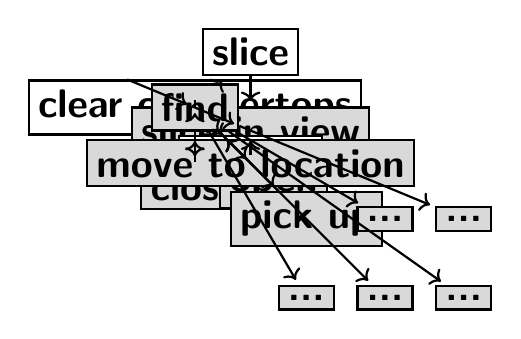
\begin{tikzpicture}[->,shorten >=2pt,auto,node distance=1cm,
        thick,main node/.style={rectangle,fill=white,draw,font=\sffamily\Large\bfseries},action node/.style={rectangle,fill=gray!30,draw,font=\sffamily\Large\bfseries}]
    
    % Nodes
    \node[main node] (1) {clear countertops};
    \node[main node] (2) [above right of=1] {slice};
    \node[action node] (3) [below of=2] {slice in view};
    \node[main node] (4) [below right of=1] {pick ...};
    \node[action node] (5) [below left of=2] {find};
    \node[action node] (6) [below left of=3] {close};
    \node[action node] (7) [right of=6] {open};
    \node[action node] (8) [below right of=5] {move to location};
    \node[action node] (9) [below right of=8] {pick up};
    \node[action node] (10) [below of=9] {...};
    \node[action node] (11) [right of=9] {...};
    \node[action node] (12) [right of=10] {...};
    \node[action node] (13) [right of=11] {...};
    \node[action node] (14) [right of=12] {...};
    
    % Edges
    \path[every node/.style={font=\sffamily\small}]
    (1) edge node {} (2)
    (1) edge node {} (3)
    (2) edge node {} (3)
    (3) edge node {} (4)
    (4) edge node {} (1)
    (1) edge node {} (5)
    (5) edge node {} (6)
    (5) edge node {} (7)
    (5) edge node {} (8)
    (5) edge node {} (9)
    (6) edge node {} (1)
    (7) edge node {} (1)
    (8) edge node {} (1)
    (9) edge node {} (1)
    (3) edge node {} (5)
    (5) edge node {} (10)
    (5) edge node {} (11)
    (5) edge node {} (12)
    (5) edge node {} (13)
    (5) edge node {} (14);
    
    \end{tikzpicture}
    \caption{Hierarchy of tasks learned. Gray nodes denote the built-in functions of the robot, and white nodes represent the tasks learned from the curriculum. For built-in actions that involve an object (e.g., close), the object must be within the field of view for the action to be taken. Special actions (i.e., done and quit) are omitted due to space constraints.}
    \label{fig:hierarchy_tasks}
\end{figure}

\end{document}